
\documentclass[convert]{standalone}

\usepackage{tikz}
\usetikzlibrary{positioning}
\usetikzlibrary{arrows}

% Defines a `datastore' shape for use in DFDs.  This inherits from a
% rectangle and only draws two horizontal lines.
\makeatletter
\pgfdeclareshape{datastore}{
  \inheritsavedanchors[from=rectangle]
  \inheritanchorborder[from=rectangle]
  \inheritanchor[from=rectangle]{center}
  \inheritanchor[from=rectangle]{base}
  \inheritanchor[from=rectangle]{north}
  \inheritanchor[from=rectangle]{north east}
  \inheritanchor[from=rectangle]{east}
  \inheritanchor[from=rectangle]{south east}
  \inheritanchor[from=rectangle]{south}
  \inheritanchor[from=rectangle]{south west}
  \inheritanchor[from=rectangle]{west}
  \inheritanchor[from=rectangle]{north west}
  \backgroundpath{
    %  store lower right in xa/ya and upper right in xb/yb
    \southwest \pgf@xa=\pgf@x \pgf@ya=\pgf@y
    \northeast \pgf@xb=\pgf@x \pgf@yb=\pgf@y
    \pgfpathmoveto{\pgfpoint{\pgf@xa}{\pgf@ya}}
    \pgfpathlineto{\pgfpoint{\pgf@xb}{\pgf@ya}}
    \pgfpathmoveto{\pgfpoint{\pgf@xa}{\pgf@yb}}
    \pgfpathlineto{\pgfpoint{\pgf@xb}{\pgf@yb}}
 }
}
\makeatother

\begin{document}
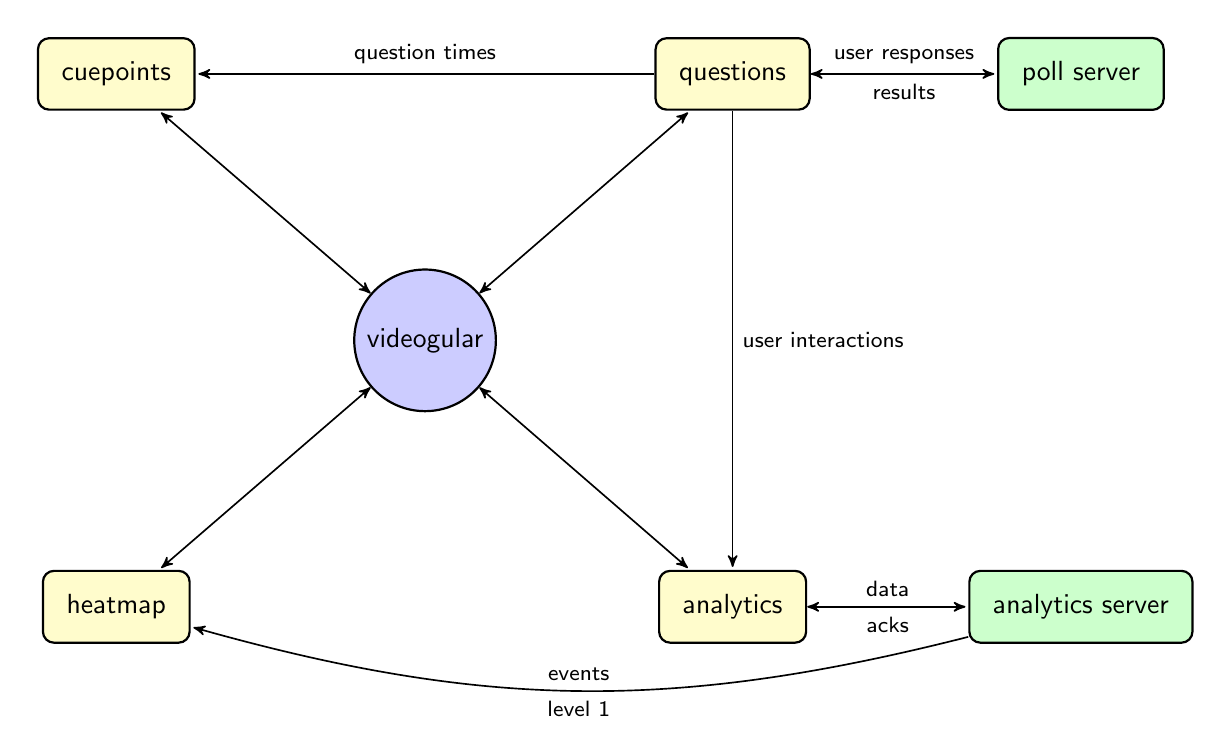
\begin{tikzpicture}[
  font=\sffamily,
  every matrix/.style={ampersand replacement=\&,column sep=2cm,row sep=2cm},
  source/.style={draw,thick,rounded corners,fill=yellow!20,inner sep=.3cm},
  vg-plugin/.style={draw,thick,rounded corners,fill=yellow!20,inner sep=.3cm},
  videogular/.style={draw,thick,circle,fill=blue!20},
  process/.style={draw,thick,circle,fill=blue!20},
  sink/.style={source,fill=green!20},
  datastore/.style={draw,very thick,shape=datastore,inner sep=.3cm},
  server/.style={source,fill=green!20},
  dots/.style={gray,scale=2},
  to/.style={->,>=stealth',shorten >=1pt,semithick,font=\sffamily\footnotesize},
  between/.style={<->,>=stealth',shorten >=1pt,semithick,font=\sffamily\footnotesize},
  every node/.style={align=center}]

  % Position the nodes using a matrix layout
  \matrix{
    \node[vg-plugin] (cuepoints) {cuepoints};
      \&
      \& \node[vg-plugin] (questions) {questions};
      \& \node[server] (poll-server) {poll server}; \\

    \& \node[videogular] (videogular) {videogular}; \\

    \node[vg-plugin] (heatmap) {heatmap};
      \&
      \& \node[vg-plugin] (analytics) {analytics};
      \& \node[server] (analytics-server) {analytics server}; \\
  };

  \draw[between] (questions) --
      node[midway,above] {user responses}
      node[midway,below] {results} (poll-server);
  \draw[to] (questions) --
      node[midway,right] {user interactions}
      (analytics);
  \draw[to] (questions) --
      node[midway,above] {question times}
      (cuepoints);
  \draw[between] (analytics) --
      node[midway,above] {data}
      node[midway,below] {acks} (analytics-server);
  \draw[to] (analytics-server) to[bend left=15] node[midway,above] {events}
      node[midway,below] {level 1} (heatmap);
  \draw[between] (videogular) -- (cuepoints);
  \draw[between] (videogular) -- (analytics);
  \draw[between] (videogular) -- (questions);
  \draw[between] (videogular) -- (heatmap);
\end{tikzpicture}

\end{document}
